\documentclass[twocolumn,onesided,9pt]{article}

\PassOptionsToPackage{table}{xcolor}

\usepackage{./Task32FlyerLatexStyle/Task32Flyer}
\usepackage{todonotes}

%% -----------------------------------
%% Document information
%% -----------------------------------
\def\pubdate{2 December 2021}
%\def\pubdate{DRAFT 1.12.2021}
\version{1.0}
\title{2021 General Meeting}
\shorttitle{2021 General Meeting}
\doctype{IEA Wind Task 32 Meeting Minutes}
\DOI{10.5281/zenodo.5718668}
%\DOI{10.5281/zenodo.xxxxxx}
\addbibresource{bibliography.bib}

%% -----------------------------------
%% Style modifications (doc specific)
%% -----------------------------------
% task 32 action box
\usepackage{tcolorbox}
\newtcolorbox{taskactions}[1][]
{
	every float=\centering,
	width=1.0\columnwidth,
	boxsep=0pt,
	left=3pt,
	right=3pt,
	top=3pt,
	colframe = Task32Blue2,
	#1,
}
% no indents
\setlength{\parindent}{0pt}
% long tables
\usepackage{supertabular}
% define figure and section references
\newcommand{\fref}[1]{Fig.~\ref{#1}}
\newcommand{\sref}[1]{\S~\ref{#1}}
% set the TOC depth
\setcounter{tocdepth}{2}
% reduce spacing in TOC
\usepackage[titles]{tocloft}
\setlength{\cftbeforesecskip}{3pt}
% authors
\newcommand{\orcid}[1]{\raisebox{6pt}{\href{https://orcid.org/#1}{
\includegraphics[width=8pt]{graphics/ORCIDiD_icon128x128.png}}}}
\usepackage{fontawesome}
\newcommand{\mailme}[1]{\raisebox{6pt}{\href{mailto:#1}{\faicon{envelope-o}}}}

%% ===================================
%:
%% Document starts
%% ===================================
\begin{document}

%% -----------------------------------
%% Title
%% -----------------------------------
\maketitle
\thispagestyle{cover}

%% -----------------------------------
%% Authors
%% -----------------------------------
\noindent\begin{minipage}{\columnwidth}
\textcolor{TextLightGrey}{Andrew Clifton,\orcid{0000-0001-9698-5083} %
    David Schlipf,\orcid{0000-0002-0189-6422}\mailme{david.schlipf@hs-flensburg.de}
%Ines Würth,\orcid{0000-0002-1365-0243}~
    Eric Simley\orcid{0000-0002-1027-9848}
}
\end{minipage}
\vskip 6pt

%% -----------------------------------
%% Introductory text
%% -----------------------------------
{\Large\noindent%
	Task 32 has created a worldwide network of wind lidar researchers who meet regularly to identify opportunities for the use of wind lidar, and mitigate the barriers to its adoption.
}
\vskip 6pt

The 2021 General Meeting took place online because of the COVID-19 pandemic. The meeting was designed to let the wind lidar community mingle virtually with their colleagues through a mix of discussion, working groups, and networking sessions.

\tableofcontents

\section*{Disclaimer}
The presence of a person’s name or company name in this document should not be taken to imply that a person or their employer agrees with any of the opinions set out here.

\newpage
% day 1
\section{Day 1: Tuesday 16 November}

\bgroup
\begin{table}[!h]
 \centering
 % set up banded rows for the agenda and add lines to the columns
 \arrayrulecolor{Task32Blue2!15}
 \rowcolors{2}{Task32Blue2!5}{white}
 \begin{tabular}{@{}|p{0.125\columnwidth}|p{0.85\columnwidth}|@{}}
 \rowcolor{Task32Blue2} \textbf{Time} & \textbf{Activity} \\
 14:00 & Introductions\\
 15:00 & Panel session on “Wind Lidar for offshore wind energy applications”\par
  \begin{tableitemize}
        \item Julia Gottschall, Fraunhofer IWES
        \item Lina Poulsen, \O rsted
        \item Adria Miquel, Eolos Floating Lidar Solutions
        \item Neil Adams, Carbon Trust
    \end{tableitemize} \\
 16:00 & Networking session\\
 16:55 & Close \\
 \end{tabular}
 \label{tab:day1-agenda}
\end{table}
\egroup

Short breaks were taken between all sessions.

\subsection{Introductions}
The day started with a short introduction to the General Meeting by the Operating Agents. This and other presentations from this meeting are available through the Task 32 Zenodo repository at \href{https://doi.org/10.5281/zenodo.5718668}{10.5281/zenodo.5718668}.

Since 2019 Task 32 has been supporting the early stage researchers (ESRs) of the Innovation Training Network Marie Skłodowska-Curie Actions: Lidar Knowledge Europe (ITN LIKE) to build their professional networks and present their work. The ESRs focus on novel techniques and the application of wind lidar for wind energy and wind engineering.

The general coordinator of ITN LIKE, Charlotte Bay Hasager (DTU Wind Energy) presented a short overview of the ITN and the ESR's work. More information about LIKE is available at \href{https://www.msca-like.eu/}{www.msca-like.eu/}. 

\faFilePowerpointO ~The presentation about the ESRs and their research interests can be found at \href{https://doi.org/10.5281/zenodo.5726900
}{DOI: 10.5281/zenodo.5726900}.

All of the other participants in the meeting then introduced themselves. 

\clearpage
\subsection{Panel discussion: “Wind Lidar for offshore wind energy applications”}

The panel included:
\begin{itemize}
        \item Julia Gottschall, Fraunhofer IWES
        \item Lina Poulsen, \O rsted
        \item Adria Miquel, Eolos Floating Lidar Solutions
        \item Neil Adams, Carbon Trust
    \end{itemize}

The panel explored the state of the art in using wind lidar for the deployment of wind energy offshore, and what R\&D are required. The discussion started with short presentations from each of the panelists about their perspectives on wind lidar for offshore wind energy applications, followed by a moderated discussion with audience questions. 75 people joined us.

Floating wind lidar have almost entirely replaced fixed-bottom met masts offshore in Europe, particularly for resource assessment. Scanning wind lidar are also used to provide data about the wind fields within operating plants, where they are placed on transformer platforms, turbine transition pieces, or the nacelle. Wind turbines are still increasing in size, with some models likely to reach 300-m tip heights in the next few years. This is within the measurement range of wind lidar, but is above the height of available validation facilities. New approaches to validation are therefore required to accurately quantify the uncertainty of wind lidar at these heights. However, it is also important to note that validation takes time; meeting climate protection goals will require speeding this up. Type certification (instead of unit certification) would help this process, but the reality is that wind lidar will seldom be the only source of data. So, it might be better to explore how to implement type certification for the entire system of wind lidar coupled with other technologies such as mesoscale modeling. As lidars replace traditional anemometers there is a growing need to use more data products derived from lidar measurements (especially turbulence intensity) to get more information about wind fields; this needs to be considered in the choice of validation methods. A lot of work is still very customer-specific rather than “off-the-shelf” and so care should be taken to develop standards and processes that allow different approaches to achieve the goals, rather than being restrictive.

\begin{taskactions}
``Accelerating offshore wind energy'' will be one of the four main themes in the relaunch of Task 32.
\end{taskactions}

\faFilePowerpointO ~ Find the presentations from the panelists in the meeting minutes at \href{https://doi.org/10.5281/zenodo.5718668}{DOI: 10.5281/zenodo.5718668}.

\subsection{ITN LIKE Poster session}

The ITN LIKE early-stage researchers provided a quick overview of their work in the plenum session, before splitting in to individual breakout rooms to discuss their work in detail.  

\begin{itemize}
\item Shahbaz Pathan, DTU Wind Energy, Denmark.
\item Liqin Jin, DTU Wind Energy, Denmark.
\item Francisco Costa, University of Stuttgart.
\item Hugo Rubio Hurtado, Fraunhofer Institute for Wind Energy Systems, University of Oldenburg.
\item Isadora Limas Coimbra, University of Porto, Faculty of Engineering.
\item Haichen Zuo, DTU Wind Energy, Denmark.
\item Jan Markus Diezel, Geophysical Institute, University of Bergen, Norway.
\item Priscila Suarez Orozco, UL International GmbH.
\item Arjun Anantharaman, Center for Wind energy research, University of Oldenburg.
\item Alessandro Sebastiani, DTU Wind Energy, Denmark.
\item Feng Guo, Flensburg University of Applied Sciences.
\item Wei Fu, DTU Wind Energy, Denmark.
\item Mohammad Nafisifard, Department of Mechanical and Structural Engineering and Material Science, University of Stavanger.
\item Zhaoyu Zhang, Department of Mechanical Engineering, Politecnico di Milano.
\item Sai Wang, University of Bergen, Norway.
\end{itemize}

More information about the ESRs and their projects are available at \href{https://www.msca-like.eu/People}{www.msca-like.eu/people}. 

\faFilePowerpointO~ Find the presentation about the ESRs and their research interests at \href{https://doi.org/10.5281/zenodo.5726900
}{DOI: 10.5281/zenodo.5726900}. 

The meeting adjourned at 16:45 CET.
% day 2
\section{Day 2: Wednesday 21 October}

\begin{table}[!h]
    \centering
    % set up banded rows for the agenda and add lines to the columns
    \arrayrulecolor{Task32Blue2!15}
    \rowcolors{2}{Task32Blue2!5}{white}
    \begin{tabular}{@{}
        |p{0.175\columnwidth-2\tabcolsep}
        |p{0.825\columnwidth-2\tabcolsep}
        |@{}}
    \rowcolor{Task32Blue2} \textbf{Time} & \textbf{Activity} \\
    14:00 & Panel session on “Wind lidar - I wish we knew how to...”:
        \begin{itemize}
            \item Mads V. Sorensen, EMD
            \item Peter Rosenbusch, Leosphere
            \item  Zachary Parker, Nordex
            \item Julia Gottschall, Fraunhofer IWES
        \end{itemize} \\
    14:55 & Break \\
    15:00 & Working groups \\
    15:55 & Break \\
    16:00 & Community news: 
        \begin{itemize}
            \item Update from the “wind lidar in cold climate” working group (Nicolas Jolin, Nergica)
            \item Update from the “wind lidar in complex terrain” working group (Alexander Stökl, Energiewerkstatt)
            \item A possible new round-robin on forward-looking lidar TI (Jens Riechert, DNV-GL)
        \end{itemize}\\
    16:45 & Close
    \end{tabular}
    \label{tab:day2-agenda}
\end{table}
\subsection{Community news}

\subsubsection{The new "Lidar data correction for sites in complex terrain (LoTar)" project}

Tobias Klaas-Witt from Fraunhofer IEE provided a short introduction to a new nationally-funded research project to create a open-source framework for modular lidar data processing. The project will build on the results of previous projects, including the Task 32 working group on ``wind lidar in complex terrain''. 

The project started in June 2021 and will run for 3 years. It is a joint project between Fraunhofer IEE and the  University of Stuttgart, who lead the project. More details can be found at \href{https://www.ifb.uni-stuttgart.de/forschung/windenergie/forschungsprojekte/LoTar/}{www.ifb.uni-stuttgart.de}.

\faFilePowerpointO ~ Find this presentation in the meeting minutes at \href{https://doi.org/10.5281/zenodo.5718668}{DOI: 10.5281/zenodo.5718668}.

\subsubsection{Update from the “wind lidar in complex terrain” working group} 

Alexander Stökl from Energiewerkstatt provided an update on this working group. Started in 2019, this group of around 10 industry and academic researchers has separately analysed data from several mountainous sites that are outside of the range of existing standards and compared them to data from meteorological towers. The results are being analysed at the moment and will be shared in a paper in 2022.

\faFilePowerpointO ~ Find this presentation in the meeting minutes at \href{https://doi.org/10.5281/zenodo.5718668}{DOI: 10.5281/zenodo.5718668}.

\subsubsection{Update from the “wind lidar in cold climate” working group} 

Marc Defossez from Nergica presented a short up date on this working group's progress. Set up in late 2020, the working group is a collaboration between Task 32 and Task 19 and will explore the opportunities and challenges for the use of wind lidar in cold climates. The group is currently identifying how it could have the most impact in this area.

Scripts to compare data from wind lidar with measurement masts were published in October 2021. They can be found in the Task 32 Github repository at \href{https://github.com/IEA-Wind-Task-32/cold-climate-data-comparison}{https://github.com/IEA-Wind-Task-32/cold-climate-data-comparison}

New participants are welcome. Please contact Marc directly for more information.

\faFilePowerpointO ~ Find this presentation in the meeting minutes at \href{https://doi.org/10.5281/zenodo.5718668}{DOI: 10.5281/zenodo.5718668}.

\subsubsection{The new round-robin on turbulence from forward-looking wind lidar}

Jakob von Eisenhart Rothe from DNV presented the plan for a round robin to compare the results from different methods of calculating turbulence intensity from a nacelle-mounted lidar. The round robin is a joint initiative between Task 32, OWC, DNV, ZX Lidars, and Leosphere.

\faFilePowerpointO ~ See details of the round robin at \href{https://doi.org/10.5281/zenodo.5713972}{DOI: 10.5281/zenodo.5713972}. The data for the round robin are available at \href{https://doi.org/10.5281/zenodo.5714038}{DOI: 10.5281/zenodo.5714038}.




\subsection{Panel discussion: \enquote{Lidar assisted control}}

The panel included:

\begin{itemize}
    \item Helena Canet, TUM. \textit{Helena’s research focuses on structural design of wind turbines. She has investigated the impact of lidar-assisted control (LAC) on wind turbine cost of energy.}
    \item Lei Liu, Goldwind. \textit{Lei Liu has five years of experience with LAC at Goldwind working on load reduction and AEP improvement. Goldwind has delivered approximately 1,000 wind turbines with LAC.}
    \item Irene Miquelez Madariaga, Public University of Navarre. \textit{Irene is working on a LAC project focusing on robust control techniques for LAC.}
    \item Steven White, ZX Lidars. \textit{ZX Lidars has 18 years of experience with nacelle and hub-mounted lidars for yaw and pitch control. Currently ZX Lidars is participating in the ReLACs lidar-assisted wind turbine control and wind farm control project.}
    \item Hailong Zhu, Movelaser. \textit{Movelaser develops nacelle-mounted lidars and has delivered approx. 2,000 units.}
\end{itemize} 

The panelists' perspectives on four main questions are summarized below:
\begin{enumerate}
    \item \textbf{What have been the main barriers for LAC so far?} 
    \begin{itemize}
        \item Clarity and consistency in understanding cost-benefit tradeoff; good lidar cost models are needed
        \item Difficulties interfacing LAC with existing turbine feedback controllers creates high entry point to use LAC; complex algorithm compared to feedback controllers, especially when considering more advanced controllers
        \item Concerns about reliability, availability, and complexity; reduction in cost of energy with LAC is very sensitive to lidar reliability and availability
        \item Need to more clearly quantify the benefit, especially because of the extra lidar costs for wind plant owners
        \item Guidance on LAC from third parties is available, but lack of standards for certification
        \item Different metrics are needed to determine how well lidars will work for LAC applications
    \end{itemize} 
    \item \textbf{What opportunities do you see for lidar in wind farm control applications?}
    \begin{itemize}
        \item Understanding the wind inflow to the wind farm can be useful, e.g., to provide forecasting for active power control applications or wake steering
        \item Additional applications beyond individual turbine control can help compensate for the cost of the lidar; but the added benefit of lidar in wind farm control applications is an open question
    \end{itemize} 
    \item \textbf{What can we do as the Lidar community to make LAC more attractive?}
    \begin{itemize}
        \item Help educate the community on the benefits of LAC; we like to talk about how difficult it is, but we should do a better job explaining easy solutions that currently exist
        \item Address the complexity of LAC by helping create standards for the design and use of LAC
        \item Make lidar easier to use for LAC by creating smart lidars that can adapt to changing atmospheric or site conditions, provide ready-to-use signals for LAC and simplifying the certification process
        \item Continue providing open-source simulation tools to make evaluating LAC more accessible
        \item Develop lidar cost models, similar to existing wind turbine cost models
    \end{itemize}
    \item \textbf{When will we reach 10k turbines running with LAC (Task 32 estimates there are currently around 1k turbines with LAC)?}
    \begin{itemize}
        \item 10k turbines with LAC are expected by 2025 (even in China alone); outside of the Chinese market it may take longer, although 10k lidars is still a very small percentage of the approximately 350k turbines currently installed worldwide
        \item As wind turbines continue to grow larger, the cost of a lidar will represent a smaller fraction of the total cost; this trend is expected to help accelerate the deployment of LAC
    \end{itemize}
\end{enumerate}
        
Additional questions from the audience:
\begin{enumerate}
    \item \textbf{What are the main obstacles to applying LAC on wind farms already in operation?}
    \begin{itemize}
        \item Usually it is harder to change a running system
        \item Retrofit solutions require a new whole process to test and certify the new control system
    \end{itemize} 
    \item \textbf{For minute-scale forecasting, fallback options are needed when lidar is unavailable (e.g., because of fog). How is lidar unavailability addressed in LAC applications?}
    \begin{itemize}
        \item For fatigue load reduction, lidar availability is not as much of a concern because the benefit will only be decreased by the fraction of time the lidar is unavailable. For extreme load reduction, very high availability is needed because harmful extreme loads could occur at any time.
        \item In some cases, the turbine may need to be shutdown when the lidar is unavailable to protect against extreme loads
        \item Lidar availability can be improved by increasing the laser energy, but this adds cost
        \item Another option discussed in the chat was adjusting the lidar processing parameters based on the signal quality to increase availability (e.g. increasing the averaging time or number of pulses for the Doppler Spectrum)
    \end{itemize}
    \item \textbf{Why are robust control techniques considered for LAC? This could make the controllers too conservative, reducing the benefits of LAC.}
    \begin{itemize}
        \item There will always be some error between what the lidar measures and the wind that interacts with the turbine. Measurement error models can be developed and accounted for in the controller design. This is different from designing a controller to be robust to all possible lidar failures at all times. Fallback options could be used instead when the lidar is unavailable.
    \end{itemize}
\end{enumerate}

\begin{taskactions}
Lidar-assisted control of wind turbines will be part of the ``universal inflow'' theme in the relaunch of Task 32.
\end{taskactions}

\subsection{Poster and networking session}

The session started with posters from Pedro Santos about the business case for scanning lidar in complex terrain, and from Axel Schild about ``Mastering the challenges of industrial lidar-assisted model predictive turbine control''. 

\faFilePowerpointO ~ Find Pedro's presentation at \href{https://doi.org/10.5281/zenodo.5713043}{DOI: 10.5281/zenodo.5713043}.

\faFilePowerpointO ~ Find Axel's presentation in the meeting minutes at \href{https://doi.org/10.5281/zenodo.5718668}{DOI: 10.5281/zenodo.5718668}.

Afterwards the participants were split randomly into breakout rooms for networking.

The meeting adjourned for the day at 16:45 CET.
% day 3
\section{Day 3: Thursday 21 October}

\begin{table}[!h]
    \centering
    % set up banded rows for the agenda and add lines to the columns
    \arrayrulecolor{Task32Blue2!15}
    \rowcolors{2}{Task32Blue2!5}{white}
    \begin{tabular}{@{}
        |p{0.175\columnwidth-2\tabcolsep}
        |p{0.825\columnwidth-2\tabcolsep}
        |@{}}
    \rowcolor{Task32Blue2} \textbf{Time} & \textbf{Activity} \\  
    14:00 & Panel session on “Wind lidar - the next generation”:
        \begin{itemize}
            \item Clym Stock-Williams, TNO
            \item Sandrine Aubrun, ECN
            \item Marijn Floris van Dooren, ForWind, Oldenburg
            \item Sarah Barber, OST
        \end{itemize} \\
    14:55 & Break \\
    15:00 & Working groups \\
    15:55 & Break \\
    16:00 & Reporting \& next steps \\
    16:45 & Close
    \end{tabular}
    \label{tab:day2-agenda}
\end{table}
\subsection{Plans for the future of Task 32}
Task 32 will reach the end of its current phase at the end of 2021. A proposal was made to the IEA Wind TCP Executive Committee (ExCo) in November 2021 to relaunch the Task. The proposal was led by Julia Gottschall from Fraunhofer IWES and David Schlipf. Julia Gottschall will replace Andrew Clifton from the University Stuttgart as the lead Operating Agent, representing the Task to the ExCo. David Schlipf will continue to be the second Operating Agent.

At the time of the Task 32 General Meeting no decision had been shared by the ExCo.

The session started with a handover from Andrew Clifton to Julia Gottschall. Julia then presented the plans for the relaunch of the Task. The plans are based on extensive consultation and have been refined in Workshops with the Task members during 2021.

The relaunched Task will focus on mitigating the challenges associated with the potential factor of five increase in the number of deployed wind lidar in the next 5 to 10 years. The relaunched Task's mission and vision have been updated accordingly:
\begin{itemize}
    \item \textbf{Mission}: We work together on research to make wind lidar the best and preferred wind measurement tool for wind energy applications
    \item \textbf{Vision}: Using wind lidar will be easy. It will bring advantages and opportunities that enable the deployment of wind energy
\end{itemize}

The Task will focus on 4 main themes. These are:
\begin{enumerate}
    \item \textbf{Universal inflow characterisation}. Working towards tools and methodologies to get and use the best information about inflow conditions to any wind turbine, anywhere.
    \item \textbf{Replacing met masts}. Creating guidelines for the selection and use of different types of wind lidar and software for site assessment.
    \item \textbf{Connecting wind lidar}. Helping users to improve measurements and extract value from their lidar(s) and data by making lidar data FAIR, enabling them to connect to an ecosystem of service providers
    \item \textbf{Accelerating offshore wind deployment}. Promoting wind lidar as a key enabling technology throughout the offshore wind project lifecycle.
\end{enumerate}

\faFilePowerpointO ~Find details of the relaunch plans at \href{https://doi.org/10.5281/zenodo.5163487
}{DOI: 10.5281/zenodo.5163487}.
\subsection{Working sessions}

The participants split into groups to refine the plans for each of the themes. The participants reviewed the existing plans, modified the deliverables, and set out timetables to work towards the deliverables. These plans will be used to get the relaunched Task moving. Each group presented their plans back to the meeting at the end of the session.
\section{Summary}
The 2021 Task 32 General Meeting brought together wind lidar researchers and end users from industry, academia, and government over three, 3-hour sessions over 3 days to explore how to identify and mitigate the barriers to the adoption of wind lidar technology for wind energy applications.

The first day was an opportunity for the Task members and the 15 ITN LIKE early stage researchers to meet other and share experience. Later panel sessions explored the use of wind lidar for offshore wind energy and the opportunities for lidar-assisted controls.

Task 32 comes to the end of its current phase in December 2021. A relaunch of the Task has been proposed to the IEA Wind ExCo and is under review. The final day of the 2021 General Meeting reviewed and revised the plans for the relaunched Task. The working groups that were active in 2021 will continue alongside new initiatives.

Task 32 and its successor welcome anyone interested in working together on research to make wind lidar the best and preferred wind measurement tool for wind energy applications. Please see \href{https://iea-wind.org/task32/}{iea-wind.org} for details.

\clearpage
\section*{List of Participants}

The following table lists people who attended part or all of the meeting. The presence of a person's name or company name in this list should not be taken to imply that a person or their employer agrees with any of the opinions set out in these minutes. We apologise for any spelling mistakes, omissions, or other errors.

% set up banded rows for the agenda and add lines to the columns
\bgroup
\tablehead{\rowcolor{Task32Blue2} \textbf{Name} & \textbf{Affiliation} \\ }
\arrayrulecolor{Task32Blue2!15}
\rowcolors{2}{Task32Blue2!5}{white}
\begin{supertabular}{@{}|p{\dimexpr 0.5\linewidth-2\tabcolsep}|p{\dimexpr 0.5\linewidth-2\tabcolsep}|@{}}
Neil Adams & Carbon Trust \\
Arjun Anantharaman & University of Oldenburg \\
Oliver Bischoff & SWE, U. Stuttgart \\
Andrew Black & Vaisala \\
Helena Canet & TUM\\
Yiyn Chen & SWE, U. Stuttgart \\
Steve Clark & NRG Systems \\
Andy Clifton & SWE, U. Stuttgart \\
Peter Clive & Black and Veatch \\
Isadora Limas Coimbra & U. Porto \\
David Collet & IFPEN \\
Francisco Costa & SWE, U. Stuttgart \\
Marie-Anne Cowan & Wood Thilsted \\
C\'edric Dall'Ozzo & EDF-RE\\
Spandan Das & ventus \\
Marc Defossez & Nergica \\
Reesa Dexter & DNV \\
Jan Markus Diezel & U. Bergen \\
Wei Fu & DTU Wind Energy \\
Paula Gomez & DTU Wind Energy \\
Julia Gottschall & Fraunhofer IWES \\
Feng Guo & DTU Wind Energy \\
Charlotte Hasager & DTU Wind Energy \\
Claudia Hodonou & Nergica \\
Adrian How & SSE \\
Poul Hummelshøj & METEK Nordic ApS \\
Masaharu Imaki & Mitsubishi Electric Corporation \\
Claudiu Ionita & Siemens Gamesa \\
Liqin Jin & DTU Wind Energy\\
Aidan Keane & Wood Renewables \\
Felix Kelberlau & Fugro \\
Tobias Klaas-Witt & Fraunhofer IEE\\
Steven Knoop & KNMI \\
Sara Koller & Meteotest \\
Nikolaos Kouris & Windar Photonics \\
Levent Kucuk & Vattenfall \\
Will Laird & Wood Plc.\\
Dexing Liu & SWE, U. Stuttgart \\
Hong Liu & engie \\
Vegar Neshaug & Fugro \\
Zachary Parker & Nordex \\
Shahbaz Pathan & DTU wind Energy \\
Mariìa Joseì Pedrayes & Vestas \\
Hugues Portevin & Leosphere \\
Lina Poulsen & \O rsted\\
Priscila Orozco & UL \\
Steffen Raach & sowento\\
Beatriz Ramos & CIEMAT \\
Joachim Reuder & U. Bergen \\
Jens Riechert & OWC \\
Hugo Rubio & Fraunhofer IWES \\
Pedro Santos & Fraunhofer IWES \\
Axel Schild & IAV GmbH\\
David Schlipf & Flensburg University of Applied Sciences \\
Alessandro Sebastiani & DTU Wind Energy \\
Eric Simley & National Renewable Energy Laboratory \\
Elliot Simon & DTU Wind Energy \\
Mikael Sj\"oholm & DTU Wind Energy \\
Chris Slinger & ZX Lidars \\
Roy Spence & RCG \\
David Stacey & Ventus \\
Alexander Stoekl & Energiewerkstatt \\
Sebastian Streitz & Nordex Group \\
I\~nigo Torres & Enel\\
Davide Trabucchi & Deutsche Windguard Consulting \\
Juan Trujillo & UL \\
Ludwig Wagner & GWU Umwelttechnik \\
Sai Wang & U. Bergen \\
Marcel Weber & Enercon \\
Maayen Wigger & ZSW \\
Ines Wuerth & SWE, U. Stuttgart \\
Zhaoyu Zhang & Politecnico di Milano \\
Hailong Zhu & movelaser\\
Demetrios Zigras & Shell \\
\hline
\end{supertabular}
\egroup
\section*{Acknowledgements}
The meeting was moderated by Andrew (Andy) Clifton, Ines W\"urth, David Schlipf, Eric Simley, and Julia Gottschall. We gratefully acknowledge the contributions of the panelists, presenters, and the working group facilitators. We also thank the participants for their willingness to share their expertise and experience, without which this Task would not be possible.

%% -----------------------------------
%% References
%% -----------------------------------
%\section*{References}
% bibliography
\label{sec:References}
\addcontentsline{toc}{section}{References}
{\small
	\printbibliography
}
\vspace*{\fill}

%% -----------------------------------
%% Outlined block of smaller text
%% -----------------------------------
\begin{tcolorbox}[width=1.0\columnwidth,
		boxsep=0pt,
		left=3pt,
		right=3pt,
		top=3pt,
		arc=0pt,
		boxrule=0.5pt,
		toprule=0.5pt,
		colback=white,
		coltext=TextGrey
	]
	{\footnotesize

		%% -----------------------------------
		%% IEA WIND AND TASK 32
		%% -----------------------------------
		
		\begin{tabular}{m{0.3\columnwidth}m{0.6\columnwidth}}
		    \multicolumn{2}{p{0.9\columnwidth}}{%
			This document was self published by IEA Wind Task 32.
			}\\
			% IEA Wind * DO NOT EDIT THIS TEXT *
			
\includegraphics[height=2cm]{graphics/IEAWind_logo.jpg}  &
			The International Energy Agency is an autonomous organisation which works to ensure reliable, affordable and clean energy for its 30 member countries and beyond. The \href{https://iea-wind.org/}{IEA Wind Technology Collaboration Programme} supports the work of 38 independent, international groups of experts that enable governments and industries from around the world to lead programmes and projects on a wide range of energy technologies and related issues.%
			\\
			% Task 32 * DO NOT EDIT THIS TEXT *
			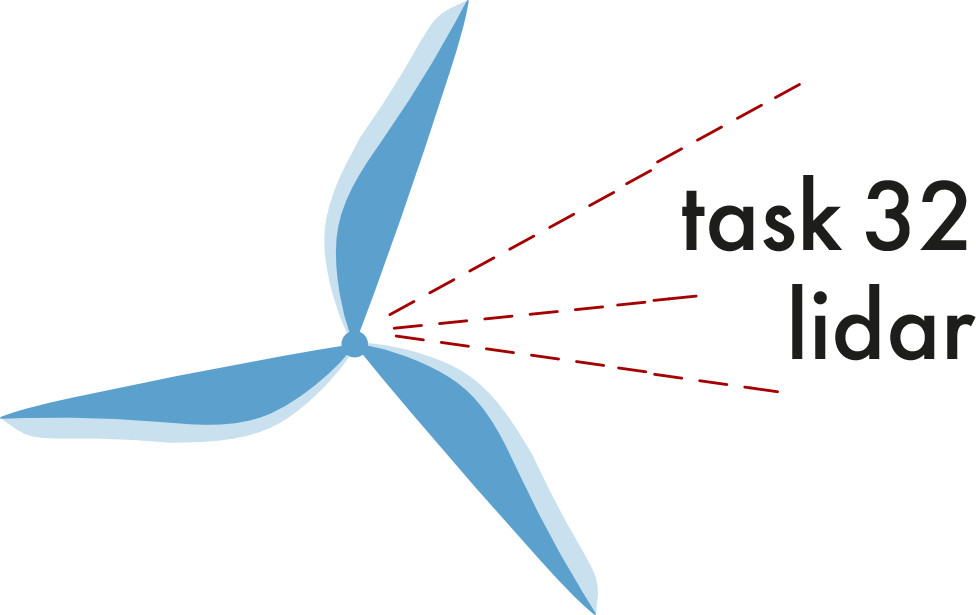
\includegraphics[height=1.5cm]{graphics/Task32_logo.jpg} &
			\href{https://iea-wind.org/task32}{IEA Wind Task 32} exists to identify and mitigate the barriers to the deployment of wind lidar for wind energy applications.\\
			% authors, etc
			\multicolumn{2}{p{0.9\columnwidth+2\tabcolsep}}{%
		%% -----------------------------------
		%% For more information
		%% -----------------------------------
		% N.B. do not add line breaks between the next items
		\textbf{For more information:} See the  \href{https://iea-wind.org/task32/}{Task 32 website}.
		%% -----------------------------------
		%% Authors
		%% -----------------------------------
		\textbf{Author team:} %
		Andrew Clifton (Task 32 Operating Agent, University of Stuttgart, Germany), %
		Ines Würth (SWE, University of Stuttgart, Germany), %		
		David Schlipf (Task 32 operating Agent, Flensburg University of Applied Sciences, Germany).
		%% -----------------------------------
		%% Reviewers
		%% -----------------------------------
		%\textbf{Reviewers:} %
		% first last (short affiliation), %
		% first last (short affiliation).
		%% -----------------------------------
		%% Images
		%% -----------------------------------
		\textbf{Images:}
		Banner, left to right: \href{https://unsplash.com/@alexkixa}{Alexandre Debiève on Unsplash}, \href{http://ifb.uni-stuttgart.de}{SWE U. Stuttgart}, \href{https://unsplash.com/@markusspiske}{Markus Spiske on Unsplash}.
	}\\
	\end{tabular}%

	}

	%% -----------------------------------
	%% End of highlighted block
	%% -----------------------------------
\end{tcolorbox}
\vspace*{\fill}

\newpage

\end{document}
